\documentclass{article}
\usepackage{amsmath,amssymb,amsthm}
\usepackage{fancyhdr}
\usepackage{enumerate}
\usepackage{float}
\usepackage{graphicx}
\usepackage{geometry}

\pagestyle{fancy}
\fancyhf{}
\lhead{Lab Exercise 2 - CSCE 221 595}
\rhead{Kevin Lei}
\renewcommand{\headrulewidth}{0.4pt}
\renewcommand{\arraystretch}{1.2}

\geometry{a4paper, margin=1in}

\begin{document}

\section*{Algorithm 1}
\begin{figure}[H]
    \centering
    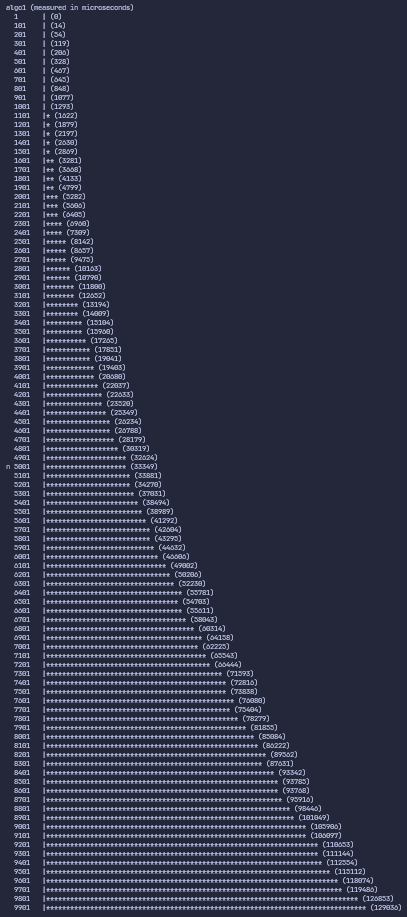
\includegraphics[width=0.5\textwidth]{./images/algo1.png}
    \caption{Graph of input size vs. time for Algorithm 1}
\end{figure}

This algorithm goes through each pair of elements in an array and checks if their sum is equal to a given target value.
The critical part of this algorithm is the nested loop, where the outer loop runs up to $n$ times ($n$ being the size of the array) and the inner loop runs up to $n-1$ times. 
This leads to a time complexity of $O(n^2)$.

\section*{Algorithm 2}
\begin{figure}[H]
    \centering
    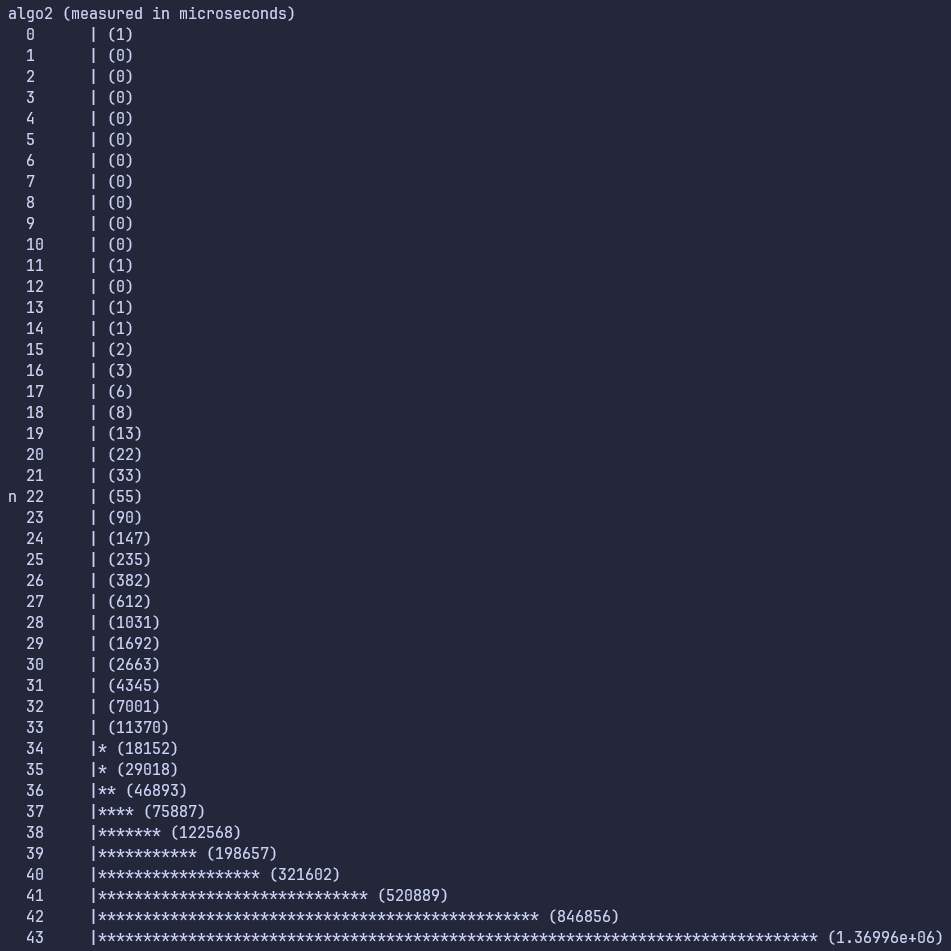
\includegraphics[width=0.5\textwidth]{./images/algo2.png}
    \caption{Graph of input size vs. time for Algorithm 2}
\end{figure}

This algorithm is a recursive implementation of the Fibonacci sequence.
The critical part of this algorithm is the recursive case, where the function calls itself twice.
Since each call to the function results in two more calls, the overall time complexity is $O(2^n)$.

\section*{Algorithm 3}
\begin{figure}[H]
    \centering
    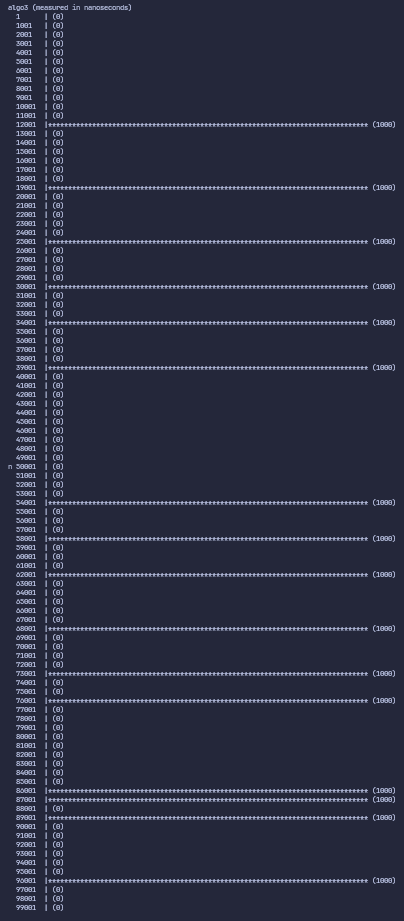
\includegraphics[width=0.5\textwidth]{./images/algo3.png}
    \caption{Graph of input size vs. time for Algorithm 3}
\end{figure}

This algorithm is an implementation of binary search.
The way this works is it checks the middle element of the current range and compares it to the target value.
If the middle element is less than the target, the algorithm searches the right half of the range, and the left half otherwise.
This process is repeated until the target value is found or the range is empty.
The critical part of this algorithm is where it halves the range, and recursively searches the left or right half.
Since each recursive call halves the range, the time complexity is $O(\log n)$.

\section*{Algorithm 4}
\begin{figure}[H]
    \centering
    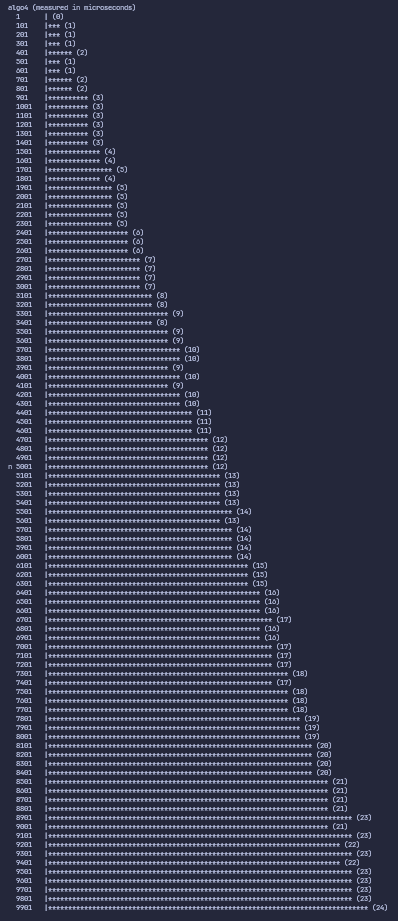
\includegraphics[width=0.5\textwidth]{./images/algo4.png}
    \caption{Graph of input size vs. time for Algorithm 4}
\end{figure}

This algorithm is just a simple linear search.
It uses a for loop to go through each element in the vector and checks if the current element is equal to the target value.
Each check will run $n$ times, where $n$ is the size of the vector, so the time complexity is $O(n)$.

\section*{Algorithm 5}
\begin{figure}[H]
    \centering
    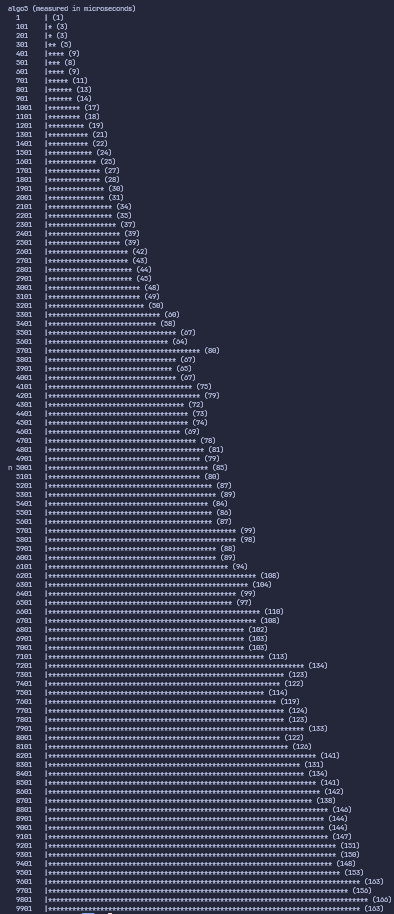
\includegraphics[width=0.5\textwidth]{./images/algo5.png}
    \caption{Graph of input size vs. time for Algorithm 5}
\end{figure}

This algorithm loops through a given vector and applies its helper function to each element, where the helper function just raises each element to the 11th power.
The critical part of this algorithm is the for loop, which runs $n$ times, and the helper function.
The way the helper function works is that it squares a recursive call to itself, and each recursive call uses a exponent that is half of the previous call.
This way, the helper function runs in $O(\log n)$ time.
However, since the exponent is fixed to 11, the time complexity of the helper function is $O(\log 11) = O(1)$, which is constant time.
So the overall time complexity of this algorithm is $O(n)$.

\end{document}
